\begin{landscape}
\vspace*{\fill}
\begin{adjustbox}{center}
%%%%%%%%%%%%%%%%%%%%%%%%%%%%%%%%%%%%%%%%%%%%%%%%%%%%%%%%%%%%%%%%
%%  UNIT RECTANGLES
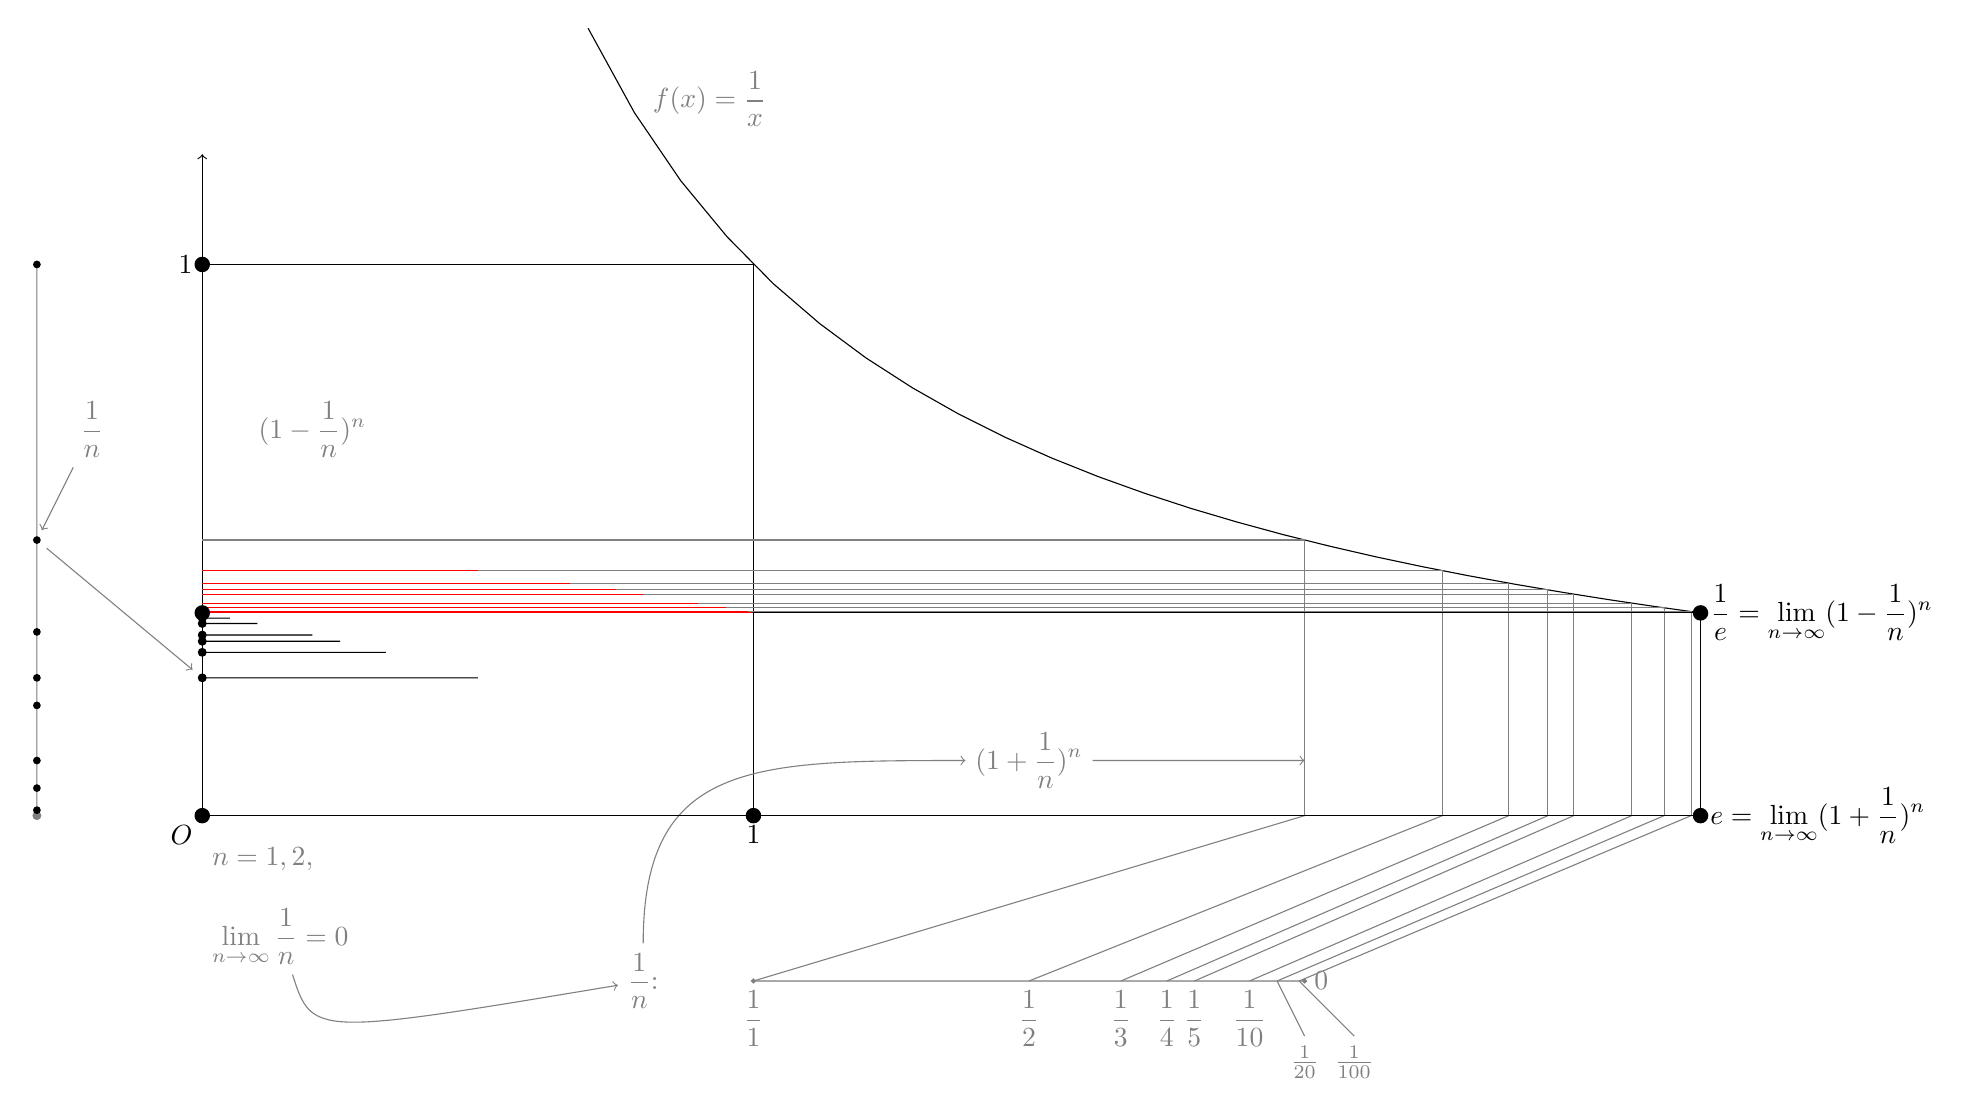
\begin{tikzpicture}[scale=7,domain=-.3:1.3]
%% \begin{tikzpicture}[xscale=5,xshift=-2,yscale=10,domain=-.3:1.3]

% \draw[very thin,color=gray] (-0.3,-0.3) grid (3.2,1.2);
%  \draw[->] (-1.2,0) -- (3.2,0) node[right] {$x$};
%  \draw[->] (0,-1.2) -- (0,2.2) node[above] {$f(x)$};

%%  f(x) = 1/x
  \draw[domain=.7:e,color=black] plot (\x,{(1/\x)});
  \draw[gray] (.8,1.3) node[right] {$f(x)=\displaystyle\frac{1}{x}$};

  %% axes
  \draw[->] (0,0) -- (0,1.2);

%% axis labels
%  \draw[black] (-0.1,.5) node %{\begin{sideways}$\displaystyle\lim_{n\to\infty}(1-\displaystyle\frac{1}{n})^n=\displaystyle\frac{1}{e}$\end{sideways}};

  \fill[black] (e,1/e) node[right]
  {$\displaystyle\frac{1}{e}=\lim_{n\to\infty}(1-\displaystyle\frac{1}{n})^n$} circle (.4pt);

  \fill[black] (e,0) node[right]
  {$e=\displaystyle\lim_{n\to\infty}(1+\frac{1}{n})^n$} circle (.4pt);

 %% dot (e,0)
%  \fill[black] (e,0) node[below] {$e$}
%  node[right=15pt] {$x=(1+\frac{1}{n})^n$}
%  circle (.4pt);


  %% indexing unit intervals
  %% horizontal
  \def\hidxv{-.3}
  \filldraw[gray] (1,\hidxv) circle (.1pt) %  node[left]  {$1$}
  -- (2,\hidxv) node[right] {$0$} circle (.1pt);

%% unit rectangles
  \draw[black] (0,0) rectangle (1,1);

% \draw[gray] (1,\hidxv) -- (2,0);
  \draw[gray] (0,\hidxv/2+0.07) node[right] (n) {$n=1,2,\dotsc$};
  \draw[gray] (0,\hidxv/2-0.07) node[right] (limninv) {$\displaystyle\lim_{n\rightarrow\infty}\frac{1}{n}=0$};
  \draw[gray] (.8,\hidxv) node (ninv) {$\displaystyle\frac{1}{n}$:};
%  -- (1,\hidxv/2)
  \draw[gray] (1.5,.1) node (eplus) {$\displaystyle (1+\frac{1}{n})^n$};
  \draw[->,gray] (eplus) -- (2,.1);

  \draw[->,gray] (limninv) .. controls (.2,-.4) .. (ninv);
  \draw[->,gray] (ninv) .. controls (.8,.1) and (1,.1) .. (eplus);

  \draw[gray] (1,\hidxv) node[below] {$\displaystyle\frac{1}{1}$} -- (2,0);

%  node[above,pos=.1] {\begin{turn}{45}$\displaystyle\frac{1}{n}\rightarrow (1+\frac{1}{n})^n$\end{turn}};
%  \draw[black] (2,0) node[below left] {$n=1$} -- (2,0);

  %% n=1
%  \draw[black] (0,0) rectangle (2,1/2); % n=1
 \draw[gray] (2,0) -- (2,1/2) -- (0,1/2);

  %% n=2
  \pgfmathsetmacro\term{(1+1/2)^2};
  \draw[gray] (\term,0) -- (\term,1/\term) -- (1-1/2,1/\term);
  \draw[color=red] (0,1/\term) -- (1-1/2,1/\term);

  \draw[gray] (1.5,\hidxv) node[below] {$\displaystyle\frac{1}{2}$} -- (\term,0);
%  \draw[gray] (1.5,\hidxv) -- (\term,0); % node[above=2pt,pos=.2]  {\begin{turn}{58}$(1+\frac{1}{2})^2$\end{turn}} ;

  %% n=3
  \pgfmathsetmacro\term{(1+1/3)^3};
  % \draw[black] (0,0) rectangle (\term,1/\term);
  \draw[gray] (\term,0) -- (\term,1/\term) -- (1-1/3,1/\term);
  \draw[color=red] (0,1/\term) -- (1-1/3,1/\term);
  \draw[gray] (2-1/3,\hidxv) node[below] {$\displaystyle\frac{1}{3}$}
  -- (\term,0); % node[above,pos=.2]  {\begin{turn}{60}$(1+\frac{1}{3})^3$\end{turn}} ;
%  \draw[black] (\term-0.03,-0.1) node[below left] {$(1+\frac{1}{3})^3$} -- (\term,0);

  \pgfmathsetmacro\term{(1+1/4)^4};
  \draw[gray] (\term,0) -- (\term,1/\term) -- (1-1/4,1/\term);
  \draw[color=red] (0,1/\term) -- (1-1/4,1/\term);
%  \draw[black] (0,0) rectangle (\term,1/\term);
  \draw[gray] (2-1/4,\hidxv) node[below] {$\displaystyle\frac{1}{4}$}
  -- (\term,0); % node[above,pos=.3]  {\begin{turn}{70}$(1+\frac{1}{4})^4$\end{turn}} ;

%  \draw[black] (\term-0.05,-0.2) node[below left] {$(1+\frac{1}{4})^4$}
%  --  (\term,0);
%  \draw[black] (-0.2,1/\term) node[left] {$(1+\frac{1}{4})^-4$} -- (0,1/\term);

  \pgfmathsetmacro\term{(1+1/5)^5};
  \draw[gray] (\term,0) -- (\term,1/\term) -- (1-1/5,1/\term);
  \draw[color=red] (0,1/\term) -- (1-1/5,1/\term);
%  \draw[black] (0,0) rectangle (\term,1/\term);
  \draw[gray] (2-1/5,\hidxv) node[below] {$\displaystyle\frac{1}{5}$}
  -- (\term,0); % node[above,pos=.3]  {\begin{turn}{60}$(1+\frac{1}{4})^4$\end{turn}} ;
%  \draw[black] (\term-0.05,-0.3) node[below] {$(1+\frac{1}{5})^5$}
%  --  (\term,0);

  \pgfmathsetmacro\term{(1+1/10)^10};
  \draw[gray] (\term,0) -- (\term,1/\term) -- (1-1/10,1/\term);
  \draw[color=red] (0,1/\term) -- (1-1/10,1/\term);
%  \draw[black] (0,0) rectangle (\term,1/\term);
  \draw[gray] (2-1/10,\hidxv) node[below] {$\displaystyle\frac{1}{10}$}
  -- (\term,0); % node[above,pos=.3]  {\begin{turn}{60}$(1+\frac{1}{4})^4$\end{turn}} ;
%  \draw[black] (\term,-0.4) node[below] {$(1+\frac{1}{10})^{10}$}
%  --  (\term,0);

  %% n=20
  \pgfmathsetmacro\term{(1+1/20)^20};
  \draw[gray] (\term,0) -- (\term,1/\term) -- (1-1/20,1/\term);
  \draw[color=red] (0,1/\term) -- (1-1/20,1/\term);
%  \draw[black] (0,0) rectangle (\term,1/\term);
  \draw[gray] (2-1/20,\hidxv) -- (\term,0);
  \draw[gray] (2-1/20+.05,\hidxv-.1) node[below] {$\frac{1}{20}$} -- (2-1/20,\hidxv);
  % node[above,pos=.3]  {\begin{turn}{60}$(1+\frac{1}{4})^4$\end{turn}} ;

  %% n=100
  \pgfmathsetmacro\term{(1+1/100)^100};
  \draw[gray] (\term,0) -- (\term,1/\term) -- (1-1/100,1/\term);
  \draw[color=red] (0,1/\term) -- (1-1/100,1/\term);
%  \draw[black] (0,0) rectangle (\term,1/\term);
  \draw[gray] (2-1/100,\hidxv) -- (\term,0);
  \draw[gray] (2-1/100+.1,\hidxv-.1) node[below] {$\frac{1}{100}$} -- (2-1/100,\hidxv);
%  \draw[black] (\term+0.1,1/\term+0.1) node[above] {$((1+\frac{1}{200})^{200},(1+\frac{1}{200})^{-200})$}
%  --  (\term,1/\term);

%%  n=infty
  \draw[black] (e,0) -- (e,1/e) -- (1,1/e);
  \draw[color=red] (0,1/e) -- (1,1/e);
  \draw[black] (0,0) -- (e,0);
%  \draw[black] (0,0) rectangle (e,1/e);

%  \draw[black] (0,1/e) -- (\e,1/e);
%  \fill[black] (0, 1/e) circle (.4pt) node[left]  {$\frac{1}{e}$};

  %% vertical
  \filldraw[gray] (-.3,0) circle (.2pt) -- (-.3,1);
  \draw[gray] (-.2,.7) node (vinv) {$\displaystyle\frac{1}{n}$};
  \draw[gray] (.2,.7) node (veinv)
  {$\displaystyle (1-\displaystyle\frac{1}{n})^n$};

  %% n=1
  \pgfmathsetmacro\term{(1-1/1)^1};
 \fill (-.3,1) node{} circle (.2pt);

 %% n=2
 \pgfmathsetmacro\term{(1-1/2)^2};
 \fill (-.3,1/2) node (vhalfidx) {} circle (.2pt);
 \filldraw (0,\term) node (vhalfax) {} circle (.2pt) -- (1/2,\term);
 \draw[->,gray] (vhalfidx) -- (vhalfax);
 \draw[->,gray] (vinv) -- (vhalfidx);
% \draw[->,gray] (veinv) -- (vhalfax);

 \pgfmathsetmacro\term{(1-1/3)^3};
 \fill (-.3,1/3) node{} circle (.2pt);
 \filldraw (0,\term) node {} circle (.2pt) -- (1/3,\term);
 
 \pgfmathsetmacro\term{(1-1/4)^4};
 \fill (-.3,1/4) node{} circle (.2pt);
 \filldraw (0,\term) node {} circle (.2pt) -- (1/4,\term);
 
 \pgfmathsetmacro\term{(1-1/5)^5};
 \fill (-.3,1/5) node{} circle (.2pt);
 \filldraw (0,\term) node {} circle (.2pt) -- (1/5,\term);

 \pgfmathsetmacro\term{(1-1/10)^10};
 \fill (-.3,1/10) node{} circle (.2pt);
 \filldraw (0,\term) node {} circle (.2pt) -- (1/10,\term);

 \pgfmathsetmacro\term{(1-1/20)^20};
 \fill (-.3,1/20) node{} circle (.2pt);
 \filldraw (0,\term) node {} circle (.2pt) -- (1/20,\term);

 \pgfmathsetmacro\term{(1-1/100)^100};
 \fill (-.3,1/100) node{} circle (.2pt);
 \filldraw (0,\term) node {} circle (.2pt) -- (1/100,\term);


  %% dot origin
  \fill[black] (0,0) node[below left] {$O$} circle (.4pt);

  %% dot (0,1/e)
 \fill[black] (0,1/e) circle (.4pt);

  %% dot (0,1)
  \fill[black] (0,1) node[left] {$1$} node[above right] {} circle (.4pt);
  %% dot (1,0)
  \fill[black] (1,0) node[below] {$1$} circle (.4pt);

%% label (1,e)
%  \fill[black] (1,e) node[anchor=south west] {$(1,e)$} circle (.4pt);

\end{tikzpicture}
\end{adjustbox}
\end{landscape}
\vfill
%%% Local Variables: 
%%% mode: latex
%%% TeX-master: t
%%% End: 
